\documentclass[12pt]{article}
\usepackage[utf8]{inputenc}
\usepackage[T1]{fontenc}
\usepackage{graphicx}
\usepackage{subcaption}
\usepackage{amsmath}
\usepackage{fancyhdr}
\usepackage{geometry}
\usepackage[english]{babel}
\usepackage{csquotes}
\usepackage{hyperref}
\usepackage{url}
\usepackage{listings}
\usepackage{float}
\usepackage{booktabs}
\usepackage{array}
\usepackage{tikz}
\usetikzlibrary{
    shapes.geometric, shapes.misc,
    arrows.meta, positioning, fit,
    backgrounds, calc, decorations.pathreplacing,
    automata
}
\usepackage{setspace}

\lstset{
    language=C,
    basicstyle=\ttfamily\small,
    numberstyle=\tiny,
    frame=single,
    breaklines=true,
}

% TikZ styles
\tikzset{
  comp/.style={rectangle, draw, rounded corners=3pt,
               minimum width=2.8cm, minimum height=0.75cm,
               align=center, font=\small},
  hw/.style={comp, fill=gray!20},
  driver/.style={comp, fill=blue!15},
  service/.style={comp, fill=green!15},
  task/.style={comp, fill=orange!20},
  app/.style={comp, fill=yellow!20},
  arr/.style={-Stealth, thick},
  biarr/.style={Stealth-Stealth, thick},
  layer/.style={rectangle, draw, minimum height=0.9cm,
                align=center, font=\small\bfseries},
  cls/.style={rectangle, draw, font=\small, text width=2.8cm,
              minimum width=3.0cm, inner sep=3pt},
  hdr/.style={cls, fill=gray!10, align=center, font=\small\bfseries},
  uses/.style={-Stealth, dashed, thick},
  impl/.style={-Stealth, thick},
  state/.style={circle, draw, fill=blue!10, minimum size=2.0cm,
                align=center, font=\small\bfseries},
}

\linespread{1.25}
\setlength{\parindent}{0.8cm}
\setlength{\parskip}{0em}
\renewcommand{\headrulewidth}{0pt}
\geometry{a4paper, portrait, margin=1in}
\setlength{\headheight}{14.49998pt}

\begin{document}
\begin{titlepage}
   \begin{center}
    \textsc{\large Ministry of Education of Republic of Moldova}\\[0.5cm]
    \textsc{\large Technical University of Moldova}\\[0.5cm]
    \textsc{\large Faculty of Computers, Informatics and Microelectronics}\\[0.5cm]
    \textsc{\large Software Engineering Department}\\[1.2cm]

    \vspace{25mm}

    {\LARGE \textbf{\textsc{Embedded Systems}}}\\[0.5cm]
    \textsc{\large Laboratory No. 1.7}\\[0.5cm]

    \newcommand{\HRule}{\rule{\linewidth}{0.5mm}}
    \vspace{80mm}

    \begin{minipage}[t]{0.4\textwidth}
    \begin{flushleft} \large
    \emph{Author:} \\
    Vladimir \textsc{Vitcovschii}\\
    std. gr. FAF-231
    \end{flushleft}
    \end{minipage}
    ~
    \begin{minipage}[t]{0.4\textwidth}
    \begin{flushright} \large
    \end{flushright}
    \end{minipage}\\[3cm]

    \vspace{5mm}
    \large Chi\c{s}in\u{a}u 2026\\[0.5cm]

    \vfill
    \end{center}
\end{titlepage}

\clearpage
\tableofcontents
\clearpage

\setcounter{page}{2}
\pagestyle{fancy}
\fancyhf{}
\rhead{\thepage}
\lhead{FAF-231 Vitcovschii Vladimir; Laboratory Work No. 1.7}

% ─────────────────────────────────────────────────────────────────────────────
\section{The Purpose of the Work}
% ─────────────────────────────────────────────────────────────────────────────

The purpose of this laboratory work is to design and implement a closed-loop automatic control application on an ATmega2560 microcontroller running FreeRTOS. The plant variable (temperature, measured by an NTC thermistor) is regulated against a configurable set point using the simplest classical regulation law: \textbf{ON-OFF control with hysteresis}. The controller drives a servo actuator (Variant~B) that switches between two saturation angles --- one for \enquote{heat} and one for \enquote{cool} --- whenever the process variable crosses the dead-band defined by the hysteresis margin. The work emphasises the modular separation of acquisition, command parsing, control, actuation, and reporting into independent FreeRTOS tasks, the use of mutex protection for shared state, and the design of an operator interface (serial line + 4$\times$4 keypad) for live set-point manipulation.

% ─────────────────────────────────────────────────────────────────────────────
\section{Objectives of the Work}
% ─────────────────────────────────────────────────────────────────────────────

The task requires implementing an ON-OFF hysteresis temperature controller on an ATmega2560 with FreeRTOS, organised as five concurrent tasks:
\begin{itemize}
  \item \textbf{Task~1 --- Acquisition}: Read the NTC thermistor via ADC every 50\,ms, convert to tenths of $^{\circ}$C through the Steinhart--Hart equation, and publish the process variable (PV) to shared memory.
  \item \textbf{Task~2 --- Command Read}: Poll the serial line and the 4$\times$4 keypad every 50\,ms; accept a numeric set point (digits + \texttt{\#}), a clear command (\texttt{*}), and four nudge keys (\texttt{A}/\texttt{B}/\texttt{C}/\texttt{D} = $\pm$1\,$^{\circ}$C\,/\,$\pm$10\,$^{\circ}$C). Update the shared set point under mutex protection.
  \item \textbf{Task~3 --- Control}: Apply the ON-OFF hysteresis law every 50\,ms. Output ON when PV $<$ SP $-$ H, OFF when PV $>$ SP $+$ H, hold previous output otherwise (the dead-band).
  \item \textbf{Task~4 --- Actuator}: Drive the servo to one of two angles (180$^{\circ}$ heat / 0$^{\circ}$ cool), refresh the green/red status LEDs, and toggle the yellow heartbeat LED.
  \item \textbf{Task~5 --- Display}: Every 500\,ms emit one Plotter-friendly tab-separated line and one human-readable status line via UART.
  \item Use a single mutex (\texttt{xLab9Mutex}) to protect every shared volatile variable.
  \item Implement temporal debouncing for digital inputs (handled by \texttt{KeypadDriver}); represent all temperatures as \texttt{int16\_t} tenths of $^{\circ}$C to avoid floating-point on AVR.
  \item Document the architecture and run the application against the test scenarios described in Section~\ref{sec:results}.
\end{itemize}

% ─────────────────────────────────────────────────────────────────────────────
\section{Domain Analysis}
% ─────────────────────────────────────────────────────────────────────────────

\subsection{Closed-Loop Automatic Control}

Automatic regulation aims to maintain a measurable physical parameter at a desired reference (\emph{set point}) in the presence of disturbances. In an embedded context the loop comprises four steps repeated periodically: sensing the process variable, computing the error against the set point, applying a control law to derive an actuation command, and driving an actuator. The cleanest separation places each step in its own software module so that the control algorithm can be replaced (ON-OFF, PID, fuzzy, etc.) without touching acquisition or actuation code.

\subsection{ON-OFF Control}

ON-OFF (\emph{bang-bang}) control is the simplest regulation strategy: the actuator is switched between exactly two states based on the comparison between the measured value and the set point. Following the lab brief \cite{labbrief}:
\begin{equation}
R(t) = \begin{cases}
K_c, & \text{if } V_{act}(t) < V_{des}(t) \\
0,   & \text{otherwise}
\end{cases}
\label{eq:onoff}
\end{equation}
where $R(t)$ is the control signal, $K_c$ is the ON command level (e.g.\ relay closed, motor on), $V_{act}$ is the measured process variable and $V_{des}$ is the set point.

The drawback is well known: at equilibrium the system oscillates rapidly around the set point, causing \emph{chattering}. Each transition stresses mechanical contacts, draws inrush current, and wears the actuator prematurely.

\subsection{Hysteresis}

Hysteresis introduces an intentional dead-band around the set point so that the control output only switches when the process variable crosses one of two thresholds, $V_{on}$ and $V_{off}$:
\begin{equation}
R(t) = \begin{cases}
K_c,     & \text{if } V_{act}(t) < V_{on}(t) \\
0,       & \text{if } V_{act}(t) > V_{off}(t) \\
R(t-1),  & \text{otherwise (hold previous output)}
\end{cases}
\label{eq:hysteresis}
\end{equation}
In this implementation the thresholds are symmetric around the set point: $V_{on} = SP - H$ and $V_{off} = SP + H$, with $H = 1.0\,^{\circ}$C. Inside the band $[SP-H, SP+H]$ the controller intentionally takes no decision, preventing the high-frequency switching.

\subsection{Output as a Function of the Process Variable}

\begin{figure}[H]
\centering
\begin{tikzpicture}[
  axis/.style={-Stealth, thick},
  out/.style={very thick, draw=blue!70!black},
  guide/.style={dashed, gray!60}
]
  \draw[axis] (-0.5,0) -- (8,0) node[right]{$V_{act}$};
  \draw[axis] (0,-0.5) -- (0,3.2) node[above]{$R(t)$};
  \node[below left] at (0,0) {$0$};

  \draw[guide] (3.2,0) -- (3.2,2.4) node[above, font=\tiny]{$V_{on}=SP-H$};
  \draw[guide] (5.2,0) -- (5.2,2.4) node[above, font=\tiny]{$V_{off}=SP+H$};

  \draw[out] (0,2.4) -- (5.2,2.4);          % top arm (ON)
  \draw[out] (5.2,2.4) -- (5.2,0.4);        % drop OFF
  \draw[out] (5.2,0.4) -- (8,0.4);          % bottom arm extension
  \draw[out] (3.2,0.4) -- (3.2,2.4);        % rise ON
  \draw[out] (0,0.4) -- (3.2,0.4);          % bottom arm

  % Arrows showing direction of traversal
  \draw[-Stealth, thick, blue!70!black] (1.5,0.4) -- ++(0.4,0);
  \draw[-Stealth, thick, blue!70!black] (3.2,1.2) -- ++(0,0.4);
  \draw[-Stealth, thick, blue!70!black] (4.5,2.4) -- ++(0.4,0);
  \draw[-Stealth, thick, blue!70!black] (5.2,1.2) -- ++(0,-0.4);

  \node[left, font=\footnotesize] at (0,2.4) {$K_c$};
  \node[left, font=\footnotesize] at (0,0.4) {$0$};
\end{tikzpicture}
\caption{Hysteresis transfer characteristic: rising and falling edges follow different paths.}
\label{fig:hysteresis}
\end{figure}

\subsection{NTC Thermistor and Steinhart--Hart Conversion}

The sensor is identical to the one used in Labs~1.5 and 1.6: a 10\,k$\Omega$ NTC thermistor with $B = 3950$ in a voltage divider with a 10\,k$\Omega$ fixed resistor. The conversion from raw 10-bit ADC code to temperature uses the Steinhart--Hart $\beta$ parameterisation; the result is scaled to tenths of $^{\circ}$C and stored as a signed 16-bit integer (\texttt{int16\_t}). Storing temperatures as integers avoids floating-point arithmetic on the ATmega2560, which has no FPU.

\subsection{Servo Actuator (Variant B)}

The lab brief offers several actuator variants; this implementation realises \textbf{Variant~B} \cite{labbrief}: a servo motor commanded via the Arduino \texttt{Servo} library on pin~D9. Although a servo is fundamentally a positional actuator, it is used here as a \emph{binary} actuator by commanding only two saturation angles: $180^{\circ}$ when the controller calls for \enquote{heat} and $0^{\circ}$ when it calls for \enquote{cool}. At boot the servo is parked at the neutral angle $90^{\circ}$. This emulates the operation of a relay or two-position valve while reusing the same hardware as Lab~1.8.

\subsection{Technology Stack}

\begin{table}[H]
\centering
\begin{tabular}{@{}lll@{}}
\toprule
\textbf{Layer} & \textbf{Technology} & \textbf{Details} \\
\midrule
Hardware Platform    & Arduino Mega 2560  & ATmega2560, 16\,MHz, 5\,V \\
Build System         & PlatformIO         & \texttt{atmelavr} platform, Arduino framework \\
Programming Language & C++                & AVR-GCC toolchain \\
RTOS                 & FreeRTOS 10.5.1    & \texttt{feilipu/FreeRTOS} Arduino library \\
Servo Library        & Arduino Servo 1.3  & \texttt{arduino-libraries/Servo} \\
STDIO Hook           & AVR-libc           & \texttt{fdev\_setup\_stream} $\to$ \texttt{SerialStream} \\
Serial Communication & UART0              & 9600\,baud, 8N1 \\
Sensor               & NTC 10\,k$\Omega$  & $B = 3950$, voltage divider with $R_{fixed} = 10$\,k$\Omega$ \\
Actuator             & Hobby servo        & PWM on D9, range 0--180$^{\circ}$ \\
Operator Interface   & 4$\times$4 keypad  & Rows D2--D5, Cols A1--A4 \\
Simulation           & Wokwi              & \texttt{diagramsWokwi/lab9/diagram.json} \\
\bottomrule
\end{tabular}
\caption{Technology Stack}
\label{tab:techstack}
\end{table}

\subsection{System Elements}

\begin{itemize}
  \item \textbf{Arduino Mega 2560 (ATmega2560)}: 256\,KB flash, 8\,KB SRAM, 16\,MHz. FreeRTOS uses one hardware timer for its tick.
  \item \textbf{NTC Thermistor (A0)}: 10\,k$\Omega$ at 25\,$^{\circ}$C, $B = 3950$. Voltage-divider topology with $R_{fixed} = 10$\,k$\Omega$.
  \item \textbf{Servo motor (D9)}: Driven via the Arduino \texttt{Servo} library. Two saturation angles $\{0, 180\}^{\circ}$ implement the binary control output.
  \item \textbf{Keypad 4$\times$4 (D2--D5 / A1--A4)}: Rows are scanned outputs, columns are pulled-up inputs. \textbf{Note:} A0 is reserved for the NTC sensor, so the keypad columns occupy A1--A4 instead of the more common A0--A3.
  \item \textbf{Green LED (D12)}: Indicates output OFF (cooling). 220\,$\Omega$ current-limiting resistor.
  \item \textbf{Red LED (D11)}: Indicates output ON (heating).
  \item \textbf{Yellow LED (D10)}: Toggles each control tick (50\,ms) as a heartbeat.
  \item \textbf{PlatformIO}: Build system; \texttt{env:mega\_lab9} environment defines \texttt{-D USE\_FREERTOS -D ACTIVE\_LAB=9}. \cite{pio}
\end{itemize}

% ─────────────────────────────────────────────────────────────────────────────
\section{Design}
% ─────────────────────────────────────────────────────────────────────────────

\subsection{Architectural Design}

The system is built from five FreeRTOS tasks communicating through a single shared-memory area protected by one mutex. Table~\ref{tab:components} lists the major components and their roles.

\begin{table}[H]
\centering
\begin{tabular}{@{}p{3.6cm}p{2.8cm}p{6.0cm}@{}}
\toprule
\textbf{Component} & \textbf{Role} & \textbf{Interface / Key Operation} \\
\midrule
NTC Thermistor (A0)  & Analog input        & 10\,k$\Omega$ NTC + voltage divider \\
NtcSensor            & Sensor driver       & \texttt{ReadNtcRaw}, \texttt{NtcAdcToTempC10} \\
Servo (D9)           & Actuator driver     & \texttt{Servo::attach}, \texttt{Servo::write} \\
LedDriver            & GPIO abstraction    & \texttt{InitializeLed}, \texttt{SetLedState} \\
KeypadDriver         & Matrix scanner      & \texttt{InitializeKeypad}, \texttt{ScanKeypad} \\
SerialStream         & UART adapter        & \texttt{IStream} over \texttt{HardwareSerial} \\
Lab9Config           & Configuration       & Pins, hysteresis, set-point bounds, intervals \\
Lab9Sync             & Shared state        & \texttt{volatile} variables + mutex handle \\
TaskAcquisition9     & Sensor task         & 50\,ms periodic ADC read \\
TaskCommandRead9     & Operator task       & 50\,ms serial + keypad parser \\
TaskControl9         & Control task        & 50\,ms ON-OFF hysteresis decision \\
TaskActuator9        & Actuator task       & 50\,ms servo + LED update \\
TaskDisplay9         & Reporting task      & 500\,ms serial status report \\
StdioRedirect        & RTE glue            & \texttt{initStdio(IStream*)} \\
MainLab9             & Entry point         & Creates mutex, tasks; starts scheduler \\
\bottomrule
\end{tabular}
\caption{Software Component Roles}
\label{tab:components}
\end{table}

\subsection{Layered Software Architecture}

\begin{figure}[H]
\centering
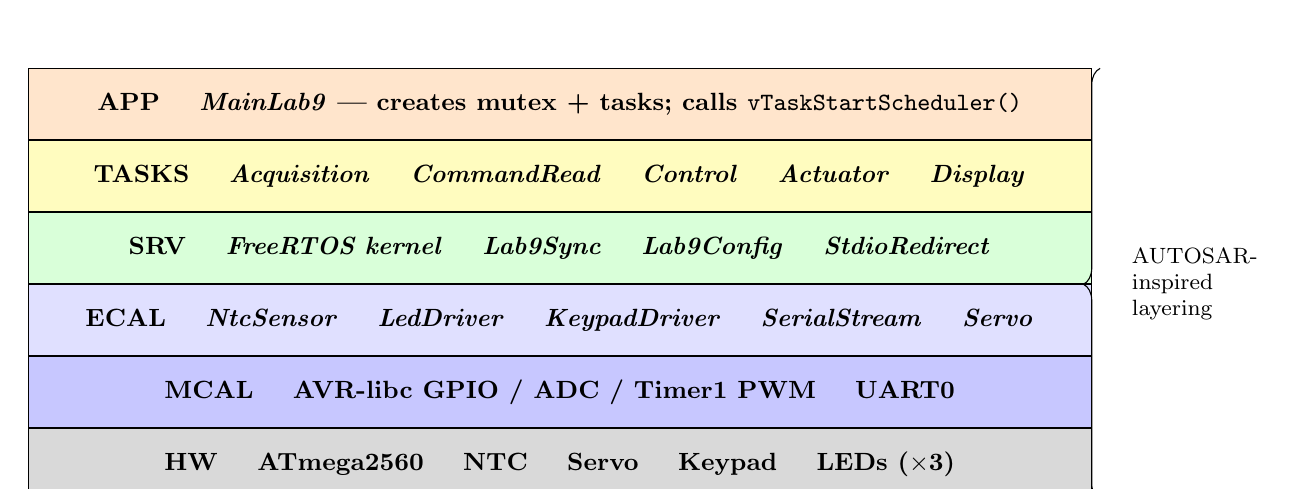
\begin{tikzpicture}[node distance=0pt]
  \def\LW{13.5cm}
  \node[layer, minimum width=\LW, fill=orange!20] (app)
    {\textbf{APP} \quad \textit{MainLab9} --- creates mutex + tasks; calls \texttt{vTaskStartScheduler()}};
  \node[layer, minimum width=\LW, fill=yellow!25, below=of app] (tasks)
    {\textbf{TASKS} \quad \textit{Acquisition} \quad \textit{CommandRead} \quad \textit{Control} \quad \textit{Actuator} \quad \textit{Display}};
  \node[layer, minimum width=\LW, fill=green!15, below=of tasks] (srv)
    {\textbf{SRV} \quad \textit{FreeRTOS kernel} \quad \textit{Lab9Sync} \quad \textit{Lab9Config} \quad \textit{StdioRedirect}};
  \node[layer, minimum width=\LW, fill=blue!12, below=of srv] (ecal)
    {\textbf{ECAL} \quad \textit{NtcSensor} \quad \textit{LedDriver} \quad \textit{KeypadDriver} \quad \textit{SerialStream} \quad \textit{Servo}};
  \node[layer, minimum width=\LW, fill=blue!22, below=of ecal] (mcal)
    {\textbf{MCAL} \quad AVR-libc GPIO / ADC / Timer1 PWM \quad UART0};
  \node[layer, minimum width=\LW, fill=gray!30, below=of mcal] (hw)
    {\textbf{HW} \quad ATmega2560 \quad NTC \quad Servo \quad Keypad \quad LEDs ($\times$3)};
  \draw[decorate, decoration={brace, amplitude=6pt, mirror}]
    ([xshift=3pt]app.north east) -- ([xshift=3pt]hw.south east)
    node[midway, right=8pt, font=\footnotesize, align=left]
    {AUTOSAR-\\inspired\\layering};
\end{tikzpicture}
\caption{Layered Software Architecture}
\label{fig:layers}
\end{figure}

\subsection{Control State Machine}

The ON-OFF hysteresis law is naturally a two-state machine. The transitions occur at the asymmetric thresholds $SP\!-\!H$ and $SP\!+\!H$.

\begin{figure}[H]
\centering
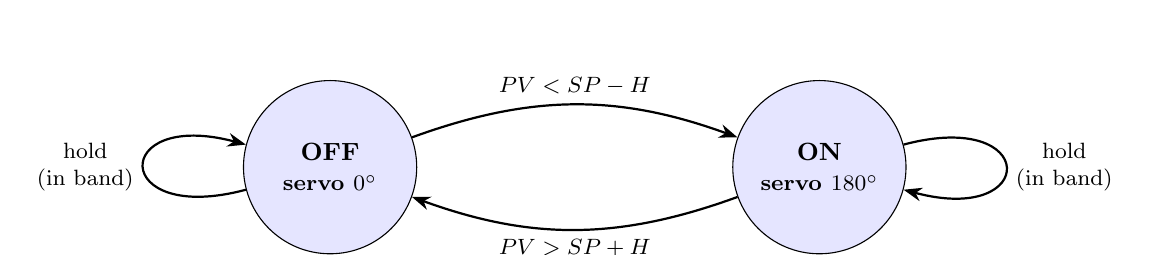
\begin{tikzpicture}[
  state/.style={circle, draw, fill=blue!10, minimum size=2.2cm,
                align=center, font=\small\bfseries},
  every loop/.style={-Stealth},
  trans/.style={-Stealth, thick}
]
  \node[state] (off) {OFF\\\footnotesize servo $0^{\circ}$};
  \node[state, right=4cm of off] (on) {ON\\\footnotesize servo $180^{\circ}$};
  \draw[trans, bend left=20] (off) to node[above, font=\footnotesize]{$PV < SP - H$} (on);
  \draw[trans, bend left=20] (on) to node[below, font=\footnotesize]{$PV > SP + H$} (off);
  \draw (off) edge[loop left, trans] node[left, font=\footnotesize, align=center]{hold\\(in band)} (off);
  \draw (on)  edge[loop right, trans] node[right, font=\footnotesize, align=center]{hold\\(in band)} (on);
\end{tikzpicture}
\caption{ON-OFF Hysteresis State Machine}
\label{fig:fsm}
\end{figure}

\subsection{Control-Loop Block Diagram}

\begin{figure}[H]
\centering
\begin{tikzpicture}[
  block/.style={rectangle, draw, rounded corners=3pt, minimum width=2.4cm, minimum height=1.0cm, align=center, font=\small},
  arr/.style={-Stealth, thick},
  node distance=1.6cm
]
  \node[block, fill=gray!20] (sp) {Set Point\\{\tiny operator}};
  \node[circle, draw, right=1.0cm of sp, minimum size=0.7cm] (sum) {$-$};
  \node[block, fill=orange!20, right=of sum] (ctrl) {ON-OFF\\Hysteresis};
  \node[block, fill=yellow!20, right=of ctrl] (act)  {Servo\\$0^{\circ}/180^{\circ}$};
  \node[block, fill=green!15, right=of act]  {Plant\\(NTC)} (plant);
  \node[block, fill=blue!15,  below=1.0cm of ctrl] (sense) {NTC + ADC\\$\to$ tenths $^{\circ}$C};
  \draw[arr] (sp) -- (sum);
  \draw[arr] (sum) -- node[above, font=\tiny]{$e=SP-PV$} (ctrl);
  \draw[arr] (ctrl) -- node[above, font=\tiny]{$R(t)$} (act);
  \draw[arr] (act) -- (plant);
  \draw[arr] (plant.south) |- node[right, font=\tiny, near end]{} (sense.east);
  \draw[arr] (sense.west) -| node[left, font=\tiny, near end]{$PV$} (sum.south);
\end{tikzpicture}
\caption{Control-Loop Block Diagram}
\label{fig:blocks}
\end{figure}

\subsection{FreeRTOS Task Synchronisation}

All five tasks share the structure shown in Figure~\ref{fig:fsm}. Synchronisation uses a single FreeRTOS mutex. There is no semaphore: the controller is purely periodic (every 50\,ms it samples the latest PV, regardless of whether a new acquisition has just completed). This keeps the design simple and predictable.

\begin{itemize}
  \item \textbf{xLab9Mutex}: Protects every shared volatile variable. Each task acquires the mutex only for the minimum duration needed --- never while doing serial I/O or hardware writes.
  \item \textbf{Priority assignment}: Acquisition (3) and CommandRead (3) run first to ensure fresh data and responsive operator interface. Control (2) and Actuator (2) follow. Display (1) is the lowest priority and yields to all other tasks.
\end{itemize}

\subsection{Electronic Design}

\begin{figure}[H]
\centering
\begin{tikzpicture}[
  blk/.style={rectangle, draw, minimum height=1.4cm, align=center, font=\small},
  mcu/.style={blk, fill=gray!15, minimum width=3.0cm, minimum height=8.5cm},
  sens/.style={blk, fill=orange!20, minimum width=2.0cm, minimum height=0.75cm},
  ledg/.style={blk, fill=green!20, minimum width=2.0cm, minimum height=0.75cm},
  ledr/.style={blk, fill=red!20,   minimum width=2.0cm, minimum height=0.75cm},
  ledy/.style={blk, fill=yellow!30, minimum width=2.0cm, minimum height=0.75cm},
  act/.style ={blk, fill=blue!20, minimum width=2.0cm, minimum height=0.75cm},
  bus/.style={-Stealth, thick},
  lbl/.style={font=\tiny, midway},
]
  \node[mcu] (mcu) {Arduino Mega\\2560\\[4pt]
    \tiny A0 $\leftarrow$ NTC\\
    A1--A4 $\leftarrow$ Keypad cols\\
    D2--D5 $\to$ Keypad rows\\
    D9 $\to$ Servo PWM\\
    D10 $\to$ Yellow LED\\
    D11 $\to$ Red LED\\
    D12 $\to$ Green LED\\
    UART0 TX/RX};

  \node[sens, left=2.6cm of mcu, yshift=2.8cm] (ntc) {NTC\\{\tiny A0, 10\,k$\Omega$ divider}};
  \node[blk, fill=gray!20, left=2.6cm of mcu, yshift=0cm, minimum width=2.0cm, minimum height=1.6cm] (kp) {Keypad 4$\times$4\\{\tiny rows D2--D5\\cols A1--A4}};

  \node[act, right=2.6cm of mcu, yshift=2.8cm] (servo) {Servo\\{\tiny D9, PWM}};
  \node[ledg, right=2.6cm of mcu, yshift=1.4cm] (gled) {Green LED\\{\tiny D12, 220\,$\Omega$}};
  \node[ledr, right=2.6cm of mcu, yshift=0.4cm] (rled) {Red LED\\{\tiny D11, 220\,$\Omega$}};
  \node[ledy, right=2.6cm of mcu, yshift=-0.6cm] (yled) {Yellow LED\\{\tiny D10, 220\,$\Omega$}};
  \node[blk, fill=blue!10, right=2.6cm of mcu, yshift=-2.0cm, minimum width=2.0cm, minimum height=0.75cm] (ser) {PC Terminal\\{\tiny UART 9600 baud}};

  \draw[bus] (ntc.east) -- node[lbl, above]{A0} (mcu.west |- ntc.east);
  \draw[bus, Stealth-Stealth] (kp.east) -- node[lbl, above]{8 pins} (mcu.west |- kp.east);
  \draw[bus] (mcu.east |- servo.west) -- node[lbl, above]{D9} (servo.west);
  \draw[bus] (mcu.east |- gled.west)  -- node[lbl, above]{D12} (gled.west);
  \draw[bus] (mcu.east |- rled.west)  -- node[lbl, above]{D11} (rled.west);
  \draw[bus] (mcu.east |- yled.west)  -- node[lbl, above]{D10} (yled.west);
  \draw[bus, Stealth-Stealth] (mcu.east |- ser.west) --
    node[lbl, above]{TX/RX} (ser.west);
\end{tikzpicture}
\caption{Electronic Design --- Pin Connection Diagram}
\label{fig:elec}
\end{figure}

\begin{itemize}
  \item \textbf{NTC Thermistor (A0)}: VCC $\to R_{fixed}$ (10\,k$\Omega$) $\to$ A0 $\to$ NTC $\to$ GND.
  \item \textbf{Servo (D9)}: PWM signal from the Arduino \texttt{Servo} library; powered from 5\,V with a common ground.
  \item \textbf{Keypad (D2--D5 / A1--A4)}: Rows configured as outputs (driven HIGH while idle); columns as \texttt{INPUT\_PULLUP}. Scanning is debounced inside \texttt{KeypadDriver}.
  \item \textbf{LEDs (D10, D11, D12)}: 220\,$\Omega$ series resistors. Green=OFF/cool, Red=ON/heat, Yellow=heartbeat.
  \item \textbf{UART0}: 9600\,baud serial connection for the 500\,ms status report and the operator command line.
\end{itemize}

% ─────────────────────────────────────────────────────────────────────────────
\section{Implementation}
% ─────────────────────────────────────────────────────────────────────────────

\subsection{Project Structure}

\begin{table}[H]
\centering
\begin{tabular}{@{}lp{8.0cm}@{}}
\toprule
\textbf{File} & \textbf{Purpose} \\
\midrule
\texttt{src/main.cpp}                       & Lab selector based on \texttt{ACTIVE\_LAB} \\
\texttt{src/labs/lab9/MainLab9.cpp}         & Defines shared state; creates mutex + 5 tasks; starts scheduler \\
\texttt{src/labs/lab9/TaskAcquisition9.cpp} & 50\,ms NTC sample $\to$ tenths $^{\circ}$C \\
\texttt{src/labs/lab9/TaskCommandRead9.cpp} & 50\,ms serial + keypad parser \\
\texttt{src/labs/lab9/TaskControl9.cpp}     & 50\,ms ON-OFF hysteresis decision \\
\texttt{src/labs/lab9/TaskActuator9.cpp}    & 50\,ms servo + LED update \\
\texttt{src/labs/lab9/TaskDisplay9.cpp}     & 500\,ms Plotter + human-readable status \\
\texttt{src/components/NtcSensor.cpp}       & ADC read, Steinhart--Hart conversion \\
\texttt{src/components/LedDriver.cpp}       & GPIO output abstraction \\
\texttt{src/components/KeypadDriver.cpp}    & 4$\times$4 matrix scanner with debouncing \\
\texttt{src/components/SerialStream.cpp}    & \texttt{IStream} over \texttt{HardwareSerial} \\
\texttt{src/components/StdioRedirect.cpp}   & \texttt{initStdio(IStream*)} \\
\texttt{include/labs/lab9/Lab9Config.h}     & Named constants: pins, hysteresis, intervals \\
\texttt{include/labs/lab9/Lab9Sync.h}       & Declares shared \texttt{volatile} data and mutex handle \\
\texttt{diagramsWokwi/lab9/diagram.json}    & Wokwi simulation circuit \\
\bottomrule
\end{tabular}
\caption{Project File Structure}
\label{tab:files}
\end{table}

\subsection{PlatformIO Environment Configuration}

\begin{lstlisting}
[env:mega_lab9]
extends = env:mega
lib_deps =
    ${env:mega.lib_deps}
    arduino-libraries/Servo@^1.3.0
    feilipu/FreeRTOS@^10.5.1-1
    fmalpartida/LiquidCrystal@^1.5.0
build_flags =
    -Wno-error=unused-variable
    -D F_CPU=16000000L
    -D USE_FREERTOS
    -D ACTIVE_LAB=9
\end{lstlisting}

\subsection{Configuration Constants}

All control-relevant values are defined as named constants in \texttt{Lab9Config.h}:

\begin{lstlisting}[caption={Lab9Config.h --- key constants}]
const uint8_t  NtcAnalogPin9      = A0;
const uint8_t  ServoPin9          = 9;
const uint8_t  GreenLedPin9       = 12;
const uint8_t  RedLedPin9         = 11;
const uint8_t  YellowLedPin9      = 10;

// Keypad: rows D2-D5, cols A1-A4 (A0 reserved for NTC)
const uint8_t  KeypadCol0Pin9     = A1;
const uint8_t  KeypadCol3Pin9     = A4;

const char     KeyCommit9         = '#';
const char     KeyClear9          = '*';
const char     KeyIncSmall9       = 'A'; // +1 C
const char     KeyDecSmall9       = 'B'; // -1 C
const char     KeyIncLarge9       = 'C'; // +10 C
const char     KeyDecLarge9       = 'D'; // -10 C

const int16_t  SetPointDefaultC10 = 250;  // 25.0 C
const int16_t  SetPointMinC10     = -100; // -10.0 C
const int16_t  SetPointMaxC10     = 500;  //  50.0 C
const int16_t  HysteresisC10      = 10;   // +/-1.0 C

const uint8_t  ServoAngleHeat9    = 180;
const uint8_t  ServoAngleCool9    = 0;
const uint8_t  ServoAngleNeutral9 = 90;

const uint16_t AcquisitionIntervalMs9 = 50;
const uint16_t ControlIntervalMs9     = 50;
const uint16_t ActuatorIntervalMs9    = 50;
const uint16_t CommandIntervalMs9     = 50;
const uint16_t DisplayIntervalMs9     = 500;
\end{lstlisting}

\subsection{Shared State and Synchronisation}

\begin{lstlisting}[caption={Lab9Sync.h --- shared volatile data and mutex}]
extern volatile uint16_t Lab9RawAdc;        // last raw ADC
extern volatile int16_t  Lab9TempC10;       // PV [tenths C]
extern volatile int16_t  Lab9SetPointC10;   // SP [tenths C]
extern volatile int16_t  Lab9HysteresisC10; // H  [tenths C]
extern volatile bool     Lab9OutputState;   // true = heating
extern volatile uint8_t  Lab9ServoAngle;    // last commanded angle

extern SemaphoreHandle_t xLab9Mutex;
\end{lstlisting}

\subsection{Setup and Scheduler Launch}

\texttt{SetupLab9()} initialises the hardware, creates the mutex and the five tasks with differentiated priorities, prints a welcome banner, and finally calls \texttt{vTaskStartScheduler()} (which never returns).

\begin{lstlisting}[caption={SetupLab9 --- task creation and scheduler launch}]
void SetupLab9() {
    SerialIo.begin(9600);
    initStdio(&SerialIo);

    InitializeNtcSensor(NtcAnalogPin9);
    InitializeLed(GreenLedPin9);
    InitializeLed(RedLedPin9);
    InitializeLed(YellowLedPin9);
    SetLedState(GreenLedPin9, true);
    SetLedState(RedLedPin9,   false);
    SetLedState(YellowLedPin9, false);

    InitializeKeypad(RowPins, ColPins);
    xLab9Mutex = xSemaphoreCreateMutex();

    xTaskCreate(TaskAcquisition9Func, "Acq",  192, nullptr, 3, nullptr);
    xTaskCreate(TaskCommandRead9Func, "Cmd",  256, nullptr, 3, nullptr);
    xTaskCreate(TaskControl9Func,     "Ctrl", 128, nullptr, 2, nullptr);
    xTaskCreate(TaskActuator9Func,    "Act",  192, nullptr, 2, nullptr);
    xTaskCreate(TaskDisplay9Func,     "Disp", 256, nullptr, 1, nullptr);

    printf_P(PSTR("Lab 9: ON-OFF Hysteresis (Variant B - servo)\n"));
    vTaskStartScheduler();
}
\end{lstlisting}

\subsection{TaskAcquisition9 --- Periodic NTC Sampling}

\begin{lstlisting}[caption={TaskAcquisition9 --- 50\,ms ADC sample $\to$ tenths $^{\circ}$C}]
void TaskAcquisition9Func(void* pv) {
    const TickType_t Interval = pdMS_TO_TICKS(AcquisitionIntervalMs9);
    TickType_t xLastWakeTime = xTaskGetTickCount();
    for (;;) {
        uint16_t raw = ReadNtcRaw(NtcAnalogPin9);
        int16_t  pv  = NtcAdcToTempC10(raw);

        xSemaphoreTake(xLab9Mutex, portMAX_DELAY);
        Lab9RawAdc  = raw;
        Lab9TempC10 = pv;
        xSemaphoreGive(xLab9Mutex);

        vTaskDelayUntil(&xLastWakeTime, Interval);
    }
}
\end{lstlisting}

\subsection{TaskControl9 --- ON-OFF Hysteresis Decision}

The control task implements Equation~\ref{eq:hysteresis} verbatim. The dead-band is enforced by the explicit \enquote{otherwise hold} branch: the variable \texttt{out} is loaded from the previous state, only updated on threshold crossing, and stored back unconditionally.

\begin{lstlisting}[caption={TaskControl9 --- hysteresis decision}]
void TaskControl9Func(void* pv) {
    const TickType_t Interval = pdMS_TO_TICKS(ControlIntervalMs9);
    TickType_t xLastWakeTime = xTaskGetTickCount();
    for (;;) {
        xSemaphoreTake(xLab9Mutex, portMAX_DELAY);
        int16_t pv   = Lab9TempC10;
        int16_t sp   = Lab9SetPointC10;
        int16_t hyst = Lab9HysteresisC10;
        bool    out  = Lab9OutputState;
        xSemaphoreGive(xLab9Mutex);

        if (pv < sp - hyst)      out = true;   // turn ON  (heating)
        else if (pv > sp + hyst) out = false;  // turn OFF (cooling)
        // else: hold previous output (dead-band)

        xSemaphoreTake(xLab9Mutex, portMAX_DELAY);
        Lab9OutputState = out;
        xSemaphoreGive(xLab9Mutex);
        vTaskDelayUntil(&xLastWakeTime, Interval);
    }
}
\end{lstlisting}

\subsection{TaskCommandRead9 --- Operator Interface}

The command task accepts two parallel input streams. Serial input expects an integer in whole degrees Celsius terminated by newline (e.g.\ \texttt{27\textbackslash n} sets SP = 27.0\,$^{\circ}$C). The keypad accumulates digits in a private buffer; \texttt{\#} commits the value, \texttt{*} clears the buffer. \texttt{A}/\texttt{B} nudge the set point by $\pm$1\,$^{\circ}$C and \texttt{C}/\texttt{D} by $\pm$10\,$^{\circ}$C. All set points are clamped to $[-10, +50]\,^{\circ}$C.

\begin{lstlisting}[caption={TaskCommandRead9 --- keypad processing}]
while (IsKeypadKeyAvailable()) {
    char key = ScanKeypad();
    if (key >= '0' && key <= '9') {
        if (keypadIdx < CmdBufferSize9 - 1) {
            keypadBuffer[keypadIdx++] = key;
            putchar(key);
        }
    } else if (key == KeyClear9) {
        keypadIdx = 0;
        printf_P(PSTR(" [cleared]\n"));
    } else if (key == KeyCommit9) {
        if (keypadIdx > 0) {
            keypadBuffer[keypadIdx] = '\0';
            long v = strtol(keypadBuffer, nullptr, 10);
            SubmitSetPoint((int16_t)(v * 10));
            keypadIdx = 0;
        }
    } else if (key == KeyIncSmall9) NudgeSetPoint(+10);
    else if   (key == KeyDecSmall9) NudgeSetPoint(-10);
    else if   (key == KeyIncLarge9) NudgeSetPoint(+100);
    else if   (key == KeyDecLarge9) NudgeSetPoint(-100);
}
\end{lstlisting}

\subsection{TaskActuator9 --- Servo and LED Update}

\begin{lstlisting}[caption={TaskActuator9 --- drive servo and update LEDs}]
void TaskActuator9Func(void* pv) {
    Lab9Servo.attach(ServoPin9);
    Lab9Servo.write(ServoAngleNeutral9);
    bool yellowBlink = false;
    for (;;) {
        xSemaphoreTake(xLab9Mutex, portMAX_DELAY);
        bool out = Lab9OutputState;
        xSemaphoreGive(xLab9Mutex);

        uint8_t angle = out ? ServoAngleHeat9 : ServoAngleCool9;
        Lab9Servo.write(angle);

        SetLedState(GreenLedPin9, !out);
        SetLedState(RedLedPin9,    out);
        yellowBlink = !yellowBlink;
        SetLedState(YellowLedPin9, yellowBlink);

        xSemaphoreTake(xLab9Mutex, portMAX_DELAY);
        Lab9ServoAngle = angle;
        xSemaphoreGive(xLab9Mutex);
        vTaskDelayUntil(&xLastWakeTime, Interval);
    }
}
\end{lstlisting}

\subsection{TaskDisplay9 --- Plotter and Status Report}

The display task emits two lines every 500\,ms. The first line is tab-separated and consumable by the Arduino IDE \emph{Serial Plotter} (each label-value pair becomes its own trace); the second is a human-readable status line.

\begin{lstlisting}[caption={TaskDisplay9 --- 500\,ms status output}]
printf_P(PSTR("SP:%d\tPV:%d\tOUT:%d\tANG:%u\n"),
    sp, pv, out ? 100 : 0, angle);
printf_P(PSTR("# SP=%d.%d C  PV=%d.%d C  H=%d.%d C  OUT=%s\n"),
    sp / 10, abs(sp) % 10,
    pv / 10, abs(pv) % 10,
    hyst / 10, abs(hyst) % 10,
    out ? "ON" : "OFF");
\end{lstlisting}

\subsection{STDIO Usage}

\begin{table}[H]
\centering
\begin{tabular}{@{}lp{4cm}p{6.0cm}@{}}
\toprule
\textbf{Function} & \textbf{Call site} & \textbf{Output} \\
\midrule
\texttt{printf\_P} & \texttt{SetupLab9} (4$\times$) & Welcome banner, sensor/actuator pins, default SP and hysteresis \\
\texttt{printf\_P} & \texttt{TaskCommandRead9}      & \texttt{[SP=...]} confirmation on every change; \texttt{[cleared]} on \texttt{*} \\
\texttt{printf\_P} & \texttt{TaskDisplay9} (2$\times$) & Plotter line + human-readable status every 500\,ms \\
\texttt{Serial.read} & \texttt{TaskCommandRead9}    & Operator integer set-point line \\
\bottomrule
\end{tabular}
\caption{STDIO Usage}
\label{tab:stdio}
\end{table}

\subsection{Code}

The complete source is available at the GitHub repository listed as the first entry in the bibliography \cite{code}.

% ─────────────────────────────────────────────────────────────────────────────
\section{Results}\label{sec:results}
% ─────────────────────────────────────────────────────────────────────────────

The application was verified on Wokwi simulation and on physical hardware. The following scenarios were tested:
\begin{enumerate}
  \item \textbf{Welcome banner}: On power-up, the firmware prints the lab title, sensor/actuator pins, default set point (\texttt{25.0\,C}) and hysteresis (\texttt{$\pm$1.0\,C}), and a one-line operator help.
  \item \textbf{Default cooling state}: With the simulated NTC at 25.0\,$^{\circ}$C and SP=25.0\,$^{\circ}$C the controller stays in the dead-band (output OFF); the green LED is on and the servo at $0^{\circ}$.
  \item \textbf{ON crossing}: Cooling the NTC below 24.0\,$^{\circ}$C (SP\,$-$\,H) drives the output ON --- the servo moves to $180^{\circ}$ and the red LED lights.
  \item \textbf{OFF crossing}: Heating the NTC above 26.0\,$^{\circ}$C (SP\,$+$\,H) drives the output OFF.
  \item \textbf{Dead-band hold}: Inside [24.0, 26.0]\,$^{\circ}$C the output retains its previous state; no chattering even when the PV oscillates inside the band.
  \item \textbf{Serial set point}: Typing \texttt{30} + \texttt{Enter} updates SP to 30.0\,$^{\circ}$C; the controller immediately re-evaluates against the new threshold pair $\{29, 31\}$.
  \item \textbf{Keypad commit}: Typing \texttt{2}, \texttt{8}, \texttt{\#} sets SP to 28.0\,$^{\circ}$C; the firmware echoes \texttt{[SP=28.0 C]}.
  \item \textbf{Keypad clear}: Typing \texttt{1}, \texttt{2}, \texttt{*} aborts the entry and prints \texttt{[cleared]}.
  \item \textbf{Nudge keys}: Pressing \texttt{A}/\texttt{B}/\texttt{C}/\texttt{D} increments / decrements SP by $\pm$1\,$^{\circ}$C / $\pm$10\,$^{\circ}$C; clamping to $[-10, +50]\,^{\circ}$C is enforced.
  \item \textbf{Yellow heartbeat}: The yellow LED toggles every 50\,ms (visible as a $\sim$10\,Hz flicker).
\end{enumerate}

A sample serial monitor output:

\begin{lstlisting}
Lab 9: ON-OFF Hysteresis (Variant B - servo)
Sensor: NTC on A0  Servo: D9
SP=25.0 C  Hyst=+/-1.0 C
Setpoint: serial 'NN' or keypad NN '#'  *=clr A/B=+/-1 C/D=+/-10
SP:250  PV:248  OUT:100  ANG:180
# SP=25.0 C  PV=24.8 C  H=1.0 C  OUT=ON
SP:250  PV:255  OUT:100  ANG:180
# SP=25.0 C  PV=25.5 C  H=1.0 C  OUT=ON
SP:250  PV:262  OUT:0    ANG:0
# SP=25.0 C  PV=26.2 C  H=1.0 C  OUT=OFF
[SP=28.0 C]
SP:280  PV:262  OUT:100  ANG:180
# SP=28.0 C  PV=26.2 C  H=1.0 C  OUT=ON
\end{lstlisting}

\subsection{Test Validation}

\begin{table}[H]
\centering
\begin{tabular}{@{}llp{7.5cm}@{}}
\toprule
\textbf{Test ID} & \textbf{Result} & \textbf{Observations} \\
\midrule
RF01\_T01  & Pass & Acquisition reads NTC every 50\,ms; PV updated under mutex. \\
RF02\_T01  & Pass & Lower threshold crossing turns output ON (servo $180^{\circ}$). \\
RF03\_T01  & Pass & Upper threshold crossing turns output OFF (servo $0^{\circ}$). \\
RF04\_T01  & Pass & Dead-band hold prevents chattering inside $[SP-H, SP+H]$. \\
RF05\_T01  & Pass & Serial integer line updates SP and is clamped to legal range. \\
RF06\_T01  & Pass & Keypad digits + \texttt{\#} commit updates SP and echoes confirmation. \\
RF07\_T01  & Pass & \texttt{*} clears keypad buffer; entry is discarded. \\
RF08\_T01  & Pass & \texttt{A}/\texttt{B}/\texttt{C}/\texttt{D} nudge SP by $\pm$1 / $\pm$10\,$^{\circ}$C. \\
RF09\_T01  & Pass & Display task emits Plotter line + human-readable line every 500\,ms. \\
RF10\_T01  & Pass & Green/Red LEDs reflect output state; yellow LED toggles each tick. \\
RNF01\_T01 & Pass & Five tasks run concurrently; no deadlock or data corruption. \\
RNF02\_T01 & Pass & Code is modular: per-task file pair; drivers reused from earlier labs. \\
RNF03\_T01 & Pass & \texttt{xLab9Mutex} protects every shared volatile variable. \\
RNF04\_T01 & Pass & All pin numbers, intervals, and thresholds are named constants. \\
RNF05\_T01 & Pass & Keypad columns A1--A4 (not A0--A3) avoid conflict with NTC. \\
RNF06\_T01 & Pass & PROGMEM strings (\texttt{printf\_P}) conserve SRAM. \\
\bottomrule
\end{tabular}
\caption{Test Results for the ON-OFF Hysteresis Application}
\label{tab:tests}
\end{table}

% ─────────────────────────────────────────────────────────────────────────────
\section{Note on AI}
% ─────────────────────────────────────────────────────────────────────────────

\hspace{0.8cm}
For this laboratory work, AI assistants such as Claude~4.7~Opus were used for explaining theoretical background (closed-loop control, hysteresis), suggesting modular decompositions, and for paraphrasing and structuring ideas in this report. All AI-generated content was reviewed against the source files and verified by running the firmware in simulation and on hardware.

% ─────────────────────────────────────────────────────────────────────────────
\section{Conclusion}
% ─────────────────────────────────────────────────────────────────────────────

\hspace{0.8cm}
This laboratory work demonstrated automatic ON-OFF temperature control with hysteresis on an ATmega2560 running FreeRTOS. The system reads an NTC thermistor, compares the conditioned process variable against an operator-configurable set point, and toggles a servo actuator (Variant~B) between two saturation angles whenever the PV crosses one of the asymmetric thresholds $SP\!\pm\!H$. Inside the dead-band the controller intentionally holds its previous output, eliminating the high-frequency chattering characteristic of pure ON-OFF control.

\hspace{0.8cm}
Five FreeRTOS tasks (Acquisition, CommandRead, Control, Actuator, Display) run on staggered priorities and communicate exclusively through shared volatile state protected by a single mutex. The architecture mirrors the layered AUTOSAR-style stack (HW $\to$ MCAL $\to$ ECAL $\to$ SRV $\to$ TASKS $\to$ APP) established in earlier labs and reuses the \texttt{NtcSensor}, \texttt{KeypadDriver}, \texttt{SerialStream}, and \texttt{LedDriver} components without modification.

\hspace{0.8cm}
The operator interface combines two redundant input channels: a serial integer line and a 4$\times$4 keypad (digits + commit/clear + four nudge keys). Because the NTC occupies analogue pin A0, the keypad columns were relocated to A1--A4 --- a small but illustrative example of how hardware constraints propagate into software configuration. The 500\,ms display task emits a tab-separated line directly compatible with the Arduino Serial Plotter, allowing the SP/PV/OUT/ANG signals to be inspected visually during tuning. Together, these elements produce a clean, demonstrable closed-loop controller and prepare the ground for the finer-grained PID regulation studied in Lab~1.8.

% ─────────────────────────────────────────────────────────────────────────────
\section{Bibliography}
% ─────────────────────────────────────────────────────────────────────────────

\begingroup
\makeatletter
\renewcommand{\section}[2]{}
\makeatother

\begin{thebibliography}{}

  \bibitem{code}
  \url{https://github.com/NeValetik/si-labs}

  \bibitem{labbrief}
  Cojuhari I., Ababii V. \textit{Embedded Systems Laboratory --- Lab~6: Automatic regulation in embedded systems}.
  Technical University of Moldova, 2025.

  \bibitem{ntc_steinhart}
  Ametherm. \textit{NTC Thermistors --- Steinhart and Hart Equation}.
  \url{https://www.ametherm.com/thermistor/ntc-thermistor-steinhart-hart-equation}

  \bibitem{freertos_mutex}
  FreeRTOS. \textit{Mutexes}.
  \url{https://www.freertos.org/Documentation/02-Kernel/02-Kernel-features/02-Queues-mutexes-and-semaphores/04-Mutexes}

  \bibitem{servo_lib}
  Arduino. \textit{Servo Library Reference}.
  \url{https://www.arduino.cc/reference/en/libraries/servo/}

  \bibitem{pio}
  PlatformIO. \textit{PlatformIO Documentation --- atmelavr Platform}.
  \url{https://docs.platformio.org/en/latest/platforms/atmelavr.html}

  \bibitem{avr}
  Microchip Technology. \textit{ATmega2560 Datasheet}, DS40002211A, 2020.
  \url{https://ww1.microchip.com/downloads/en/devicedoc/atmel-2549-8-bit-avr-microcontroller-atmega640-1280-1281-2560-2561_datasheet.pdf}

\end{thebibliography}
\endgroup

\pagebreak
\end{document}
